\section{Functions of Several Variables and Three Dimensional Space} \label{S:9.1.Functions}

\vspace*{-14 pt}
\framebox{\hspace*{3 pt}
\parbox{6.25 in}{\begin{goals}
%\item What is the difference between a left-hand system and a right-hand system? Why is there a difference?
\item What is a function of several variables?  What do we mean by the domain of a function of several variables?
\item How do we find the distance between two points in $\R^3$? What is the equation of a sphere in $\R^3$?
\item What is a trace of a function of two variables? What does a trace tell us about a function?
\item What is a level curve of a function of two variables? What does a level curve tell us about a function?
\end{goals}} \hspace*{3 pt}}

\subsection*{Introduction}

Throughout our mathematical careers we have studied functions of a
single variable. We define a function of one variable as a rule that
assigns exactly one output to each input. We analyze these functions
by looking at their graphs, calculating limits, differentiating,
integrating, and more. In this and following sections, we will study
functions whose input is defined in terms of more than one variable,
and then analyze these functions by looking at their graphs,
calculating limits, differentiating, integrating, and more. We will
see that many of the ideas from single variable calculus translate
well to functions of several variables, but we will have to make some
adjustments as well.

\input{previews/9.1.PA1}

\subsection*{Functions of Several Variables}

Suppose we launch a projectile, using a golf club, a cannon, or some
other device, from ground level. Under ideal conditions (ignoring wind
resistance, spin, or any other forces except the force of gravity) the
horizontal distance the object will travel depends on the initial
velocity $x$ the object is given, and the angle $y$ at which it is
launched. If we let $f$ represent the horizontal distance the object
travels (its range), then $f$ is a function of the two variables $x$
and $y$, and we represent $f$ in functional notation by
\[f(x,y) = \frac{x^2 \sin(2 y)}{g},\] where $g$ is the acceleration
due to gravity.\footnote{We will derive this equation in a later section.}

\vspace*{5pt}
\nin \framebox{\hspace*{3 pt}
\parbox{6.25 in}{\begin{definition} A \textbf{function $f$ of two independent variables}\index{function!of two variables} is a rule that assigns to each ordered pair $(x,y)$ in some set $D$ exactly one real number $f(x,y)$. \end{definition}
} \hspace*{3 pt}}
\vspace*{5pt}


There is, of course, no reason to restrict ourselves to functions of
only two variables---we can use any number of variables we like. For
example,
\[f(x,y,z) = x^2 - 2xz + \cos(y)\] 
defines $f$ as a function of the
three variables $x$, $y$, and $z$. In general, a function of $n$
independent variables is a rule that assigns to an ordered $n$-tuple
$(x_1, x_2, \ldots, x_n)$ in some set $D$ exactly one real number.

As with functions of a single variable, it is important to understand
the set of inputs for which the function is defined.

\vspace*{5pt}
\nin \framebox{\hspace*{3 pt}
  \parbox{6.25 in}{\begin{definition} The
      \textbf{domain}\index{function!domain} of a function $f$ is the
      set of all inputs at which the function is
      defined. \end{definition} } \hspace*{3 pt}} \vspace*{5pt}

\begin{activity} \label{A:9.1.1}  Identify the domain of each of the following functions. Draw a picture of each domain in the $x$-$y$ plane.
    \ba
    \item $f(x,y) = x^2+y^2$

    \item $f(x,y) = \sqrt{x^2+y^2}$

    \item $Q(x,y) = \frac{x+y}{x^2-y^2}$

    \item $s(x,y) = \frac{1}{\sqrt{1-xy^2}}$

    \ea
\end{activity}

\begin{smallhint}
\ba
\item What is the domain of a polynomial?
\item What is the domain of the square root function?
\item Under what conditions is a fraction undefined?
\item Under what conditions is a fraction undefined?
\ea
\end{smallhint}

\begin{bighint}
\ba
\item What are the domains of the functions defined by $g(x)=x^2$ and $h(y)=y^2$? 
\item What is the domain of the square root function?
\item When is $x^2-y^2=0$? 
\item When is $\sqrt{1-xy^2} > 0$?
\ea
\end{bighint}

\begin{activitySolution}
\ba
\item Since $x^2$ and $y^2$ are both polynomials, they are defined for all values of $x$ and $y$. So the domain of $f(x,y) = x^2+y^2$ is all ordered pairs of real numbers, or the entire plane. 
\item The square root of a real number is real only for nonnegative real numbers So $f(x,y) = \sqrt{x^2+y^2}$ is defined only when the argument $x^2+y^2$ of the square root is nonnegative. Now $x^2+y^2$ can never be negative, so the domain of $f(x,y) = \sqrt{x^2+y^2}$ is all ordered pairs of real numbers, or the entire plane. 
\item A fraction is undefined when the denominator is 0. So $Q(x,y) = \frac{x+y}{x^2-y^2}$ is defined for all pairs $(x,y)$ as long as $x^2-y^2 \neq 0$. Now $x^2-y^2=0$ when $y^2=x^2$ or when $\mid y \mid = \mid x \mid$. This happens along the lines $y=x$ and $y=-x$. So the domain of $Q(x,y) = \frac{x+y}{x^2-y^2}$ is all ordered pairs $(x,y)$ except for those where $y=x$ or $y=-x$.  
\item A fraction is undefined when the denominator is 0. So $s(x,y) = \frac{1}{\sqrt{1-xy^2}}$ is defined for all pairs $(x,y)$ as long as $\sqrt{1-xy^2} \neq 0$. This will happen as long as $1-xy^2 \neq 0$. In order for the square root to return a real number, we also need to have $1-xy^2 \geq 0$. Now $1-xy^2 > 0$ when $x < \frac{1}{y^2}$. So the domain of $s(x,y) = \frac{1}{\sqrt{1-xy^2}}$ is all ordered pairs $(x,y)$ so that $x < \frac{1}{y^2}$. 
\ea
\end{activitySolution}

\aftera 

\subsection*{Representing Functions of Two Variables}

One of the techniques we use to study functions of one
variable is to create a table of values. We can do the same for
functions of two variables, except that our tables will have to allow
us to keep track of both input variables. We can do this with a
2-dimensional table, where we list the $x$-values across the first row 
and the $y$-values down the first column. Let $f$ be the function
defined by $f(x,y) = \frac{x^2 \sin(2y)}{g}$ that gives the range of a
projectile as a function of the initial velocity $x$ and launch angle
$y$ of the projectile. The value $f(x,y)$ is then displayed in the
location where the $x$ row intersects the $y$ column, as shown in
Table \ref{T:9.1.range} (where we measure $x$ in feet and $y$ in
radians).

\begin{table}[ht]
\begin{center}
\begin{tabular}{|c|c|c|c|c|c|c|c|} \hline
$x\backslash y$   &$0.2$ 	&$0.4$ 	&$0.6$ 	&$0.8$ 	&$1.0$ 	&$1.2$ &$1.4$      \\ \hhline{|=|=|=|=|=|=|=|=|}
25       &7.6		&14.0	&18.2	&19.5	&17.8	&13.2	&6.5      \\ \hline
50       &30.4		&56.0	&72.8	&78.1	&71.0	&52.8	&26.2     \\ \hline
75       &68.4		&126.1	&163.8	&175.7	&159.8	&118.7	&58.9   \\ \hline
100      &121.7	&224.2	&291.3	&312.4	&284.2	&211.1	&104.7    \\ \hline
125      &190.1	&350.3	&455.1	&488.1	&444.0	&329.8	&163.6    \\ \hline
150      &273.8	&504.4	&655.3	&702.8	&639.3	&474.9	&235.5    \\ \hline
175      &372.7	&686.5	&892.0	&956.6	&870.2	&646.4	&320.6    \\ \hline
200      &486.8	&896.7	&1165.0	&1249.5	&1136.6	&844.3	&418.7    \\ \hline
225      &616.2	&1134.9	&1474.5	&1581.4	&1438.5	&1068.6	&530.0   \\ \hline
250      &           &           &           &           &           &           &                  \\ \hline
%250     &760.6	&1401.1	&1820.4	&1952.3	&1776.0	&1319.3	&654.3  \\ \hline
\end{tabular}
\caption{Values of $f(x,y) = \frac{x^2 \sin(2y)}{g}$.}
\label{T:9.1.range}
\end{center}
\end{table}

%\begin{table}[ht]
%\begin{center}
%\begin{tabular}{|c||c|c|c|c|c|c|c|c|c|c|}
%  \hline
%  $y\backslash x$ &25&50&75&100&125&150&175&200&225&250\\ \hhline{|=|=|=|}
% \hline
%  \hline
%  0.2&7.6&30.4&68.5&121.7&190.1&273.8&372.7&486.8&616.1&\hspace*{0.75in}\\
%  \hline
%  0.4&14.0&56.0&126.1&224.2&350.3&504.4&686.5&896.7&1134.9&\\
%  \hline
%  0.6&18.2&72.8&163.8&291.3&455.1&655.3&892.0&1165.0&1474.5&\\
%  \hline
%  0.8&19.5&78.1&175.7&312.4&488.1&702.8&956.6&1249.5&1581.4&\\
%  \hline
%  1.0&17.8&71.0&159.8&284.2&444.0&639.3&870.2&1136.6&1438.5&\\
%  \hline
%  1.2&13.2&52.8&118.7&211.1&329.8&474.9&646.4&844.3&1068.6&\\
%  \hline
%  1.4&6.5&26.2&58.9&104.7&163.6&235.5&320.6&418.7&530.0&\\
%  \hline
%\end{tabular}
%\caption{Values of $f(x,y) = \frac{x^2 \sin(2y)}{g}$.}
%\label{T:9.1.range}
%\end{center}
%\end{table}


\begin{activity} \label{A:9.1.2} Complete the last row in
  Table~\ref{T:9.1.range} to provide the needed values of the function
  $f$. 
  % $f(x,y) = \frac{x^2 \sin(2y)}{g}$.

\end{activity}
\begin{smallhint}
Evaluate $f$ at the points indicated by the table.
\end{smallhint}
\begin{bighint}
  The values of $x$ are read across the rows and the values of $y$
  down the columns.
\end{bighint}
\begin{activitySolution}

The entries across the last row are $f\left(250,0.2\right)$, $f\left(250,0.4\right)$, $f\left(250,0.6\right)$, $f\left(250,0.8\right)$, $f\left(250,1.0\right)$, $f\left(250,1.2\right)$, and $f\left(250,1.4\right)$. These values complete the table as shown below. 
\begin{center}
\begin{tabular}{|c|c|c|c|c|c|c|c|} \hline
$x\backslash y$   &$0.2$ 	&$0.4$ 	&$0.6$ 	&$0.8$ 	&$1.0$ 	&$1.2$ &$1.4$      \\ \hhline{|=|=|=|=|=|=|=|=|}
25       &7.6		&14.0	&18.2	&19.5	&17.8	&13.2	&6.5      \\ \hline
50       &30.4		&56.0	&72.8	&78.1	&71.0	&52.8	&26.2     \\ \hline
75       &68.4		&126.1	&163.8	&175.7	&159.8	&118.7	&58.9   \\ \hline
100      &121.7	&224.2	&291.3	&312.4	&284.2	&211.1	&104.7    \\ \hline
125      &190.1	&350.3	&455.1	&488.1	&444.0	&329.8	&163.6    \\ \hline
150      &273.8	&504.4	&655.3	&702.8	&639.3	&474.9	&235.5    \\ \hline
175      &372.7	&686.5	&892.0	&956.6	&870.2	&646.4	&320.6    \\ \hline
200      &486.8	&896.7	&1165.0	&1249.5	&1136.6	&844.3	&418.7    \\ \hline
225      &616.2	&1134.9	&1474.5	&1581.4	&1438.5	&1068.6	&530.0   \\ \hline
%250      &           &           &           &           &           &           &                  \\ \hline
250     &760.6		&1401.1	&1820.4	&1952.3	&1776.0	&1319.3	&654.3  \\ \hline
\end{tabular}
\end{center}

% \begin{center}
% \begin{tabular}{|c|c|c|c|c|c|c|c|c|} \hline
%   &$\frac{2\pi}{20}$ &$\frac{3\pi}{20}$ &$\frac{4\pi}{20}$ &$\frac{5\pi}{20}$ &$\frac{6\pi}{20}$ &$\frac{7\pi}{20}$ &$\frac{8\pi}{20}$ &$\frac{9\pi}{20}$     \\ \hline
% 25       &11.480     &15.801     &18.575     &19.531     &18.575     &15.801     &11.480     &6.0356      \\ \hline
% 50       &45.921     &63.205     &74.301     &78.125     &74.301     &63.205     &45.921     &24.142      \\ \hline
% 75       &103.322    &142.210    &167.178    &175.781    &167.178    &142.210    &103.322    &54.319    \\ \hline
% 100      &183.683    &252.818    &297.205    &312.500    &297.205    &252.818    &183.683    &96.568     \\ \hline
% 125      &287.005    &395.028    &464.383    &488.281    &464.383    &395.028    &287.005    &150.887    \\ \hline
% 150      &413.287    &568.840    &668.712    &703.125    &668.712    &568.840    &413.287    &217.278     \\ \hline
% 175      &562.529    &774.255    &910.191    &957.031    &910.191    &774.255    &562.529    &295.739    \\ \hline
% 200      &734.732    &1011.271   &1188.821   &1250.000   &1188.821   &1011.271   &734.732    &386.271     \\ \hline
% 225      &929.895    &1279.890   &1504.601   &1582.031   &1504.601   &1279.890   &929.895    &488.875     \\ \hline
% 250     &1148.018   &1580.112   &1857.532   &1953.125   &1857.532   &1580.112   &1148.018   &603.549  \\ \hline
% \end{tabular}
% \end{center}

\end{activitySolution}
\aftera

If $f$ is a function of a single variable $x$, then we define the
graph of $f$ to be the set of points of the form $(x,f(x))$, where $x$
is in the domain of $f$. We then plot these points using the
coordinate axes in order to visualize the graph. We can do a similar
thing with functions of several variables. Table \ref{T:9.1.range}
identifies points of the form $(x,y,f(x,y))$, and we define the graph
of $f$ to be the set of these points.

 \vspace*{5pt}
\nin \framebox{\hspace*{3 pt}
\parbox{6.25 in}{\begin{definition} The \textbf{graph}\index{function!graph} of a function $f = f(x,y)$ is the set of points of the form $(x,y,f(x,y))$, where the point $(x,y)$ is in the domain of $f$. \end{definition}
} \hspace*{3 pt}}
\vspace*{5pt}

We also often refer to the graph of a function $f$ of two variables as
the \emph{surface}\index{function!surface} generated by $f$. Points in
the form $(x,y,f(x,y))$ are in three dimensions, so plotting these
points takes a bit more work than graphs of functions in two
dimensions. To plot these three-dimensional points, we need to set up
a coordinate system with three mutually perpendicular axes -- the
$x$-axis, the $y$-axis, and the $z$-axis (called the \emph{coordinate
  axes}). There are essentially two different ways we could set up a
3D coordinate system, as shown in Figures \ref{F:9.1.right_hand} and
\ref{F:9.1.left_hand}; thus, before we can proceed, we need to
establish a convention.

\begin{figure}[ht]
\begin{center}
\begin{minipage}{2.5in}
\begin{center}
%\resizebox{!}{1.5in}{\includegraphics{9_1_right_hand_system}}
  \includegraphics{figures/fig_9_1_right_hand.eps}
\caption{A right hand system}
\label{F:9.1.right_hand}
\end{center}
\end{minipage}
\hspace{0.5in}
\begin{minipage}{2.5in}
\begin{center}
%\resizebox{!}{1.5in}{\includegraphics{9_1_left_hand_system}}
  \includegraphics{figures/fig_9_1_left_hand.eps}
\caption{A left hand system}
\label{F:9.1.left_hand}
\end{center}
\end{minipage}
\end{center}
\end{figure}

The distinction between these two figures is subtle, but important.
In the coordinate system shown in \ref{F:9.1.right_hand}, imagine that
you are sitting on the positive $z$-axis next to the label ``$z$.''
Looking down at the $x$- and $y$-axes, you see that the $y$-axis is
obtained by rotating the $x$-axis by 90$^\circ$ in the {\em
  counterclockwise} direction.  Again sitting on the positive $z$-axis
in Figure \ref{F:9.1.left_hand}, you see that the $y$-axis is obtained
by rotating the $x$-axis by 90$^\circ$ in the {\em clockwise}
direction.


We call the coordinate system in \ref{F:9.1.right_hand} a {\em
  right-hand system}; if we point the index finger of our {\em right}
hand along the positive $x$-axis and our middle finger along the
positive $y$-axis, then our thumb points in the direction of the
positive $z$-axis.  Following mathematical conventions, we choose to
use a right-hand system throughout this book.

% We will adopt a right-hand system\index{right hand system}, as illustrated in Figure \ref{F:9.1.right_hand}. To see the difference, think about a socket wrench -- a tool for driving screws. It consists of a handle and a socket. The socket is placed on the screw and attached to the handle. As the handle of the wrench is turned, the socket provides a force that drives the screw. If you point the index finger of your right hand in the direction of the force you apply to the handle of the wrench, and point your middle finger in the direction of the handle toward the socket, then your thumb will point in the direction in which the wrench is driving the screw. If you use your left hand instead, then your thumb will point in the opposite direction. So the socket wrench is set up to drive right-handed screws. This is exactly the 3D coordinate system we want to adopt. In a right hand system, if we point the index finger of our right hand in the direction of the positive $x$-axis and our middle finger in the direction of the positive $y$-axis, then our thumb will point in the direction of the positive $z$-axis. A left hand system and a right hand system have different orientations, so we need pick one as a standard so that the convention of orientation is understood by everyone. We will always use a right-hand system.

Now that we have established a convention for a right hand system, we can draw a graph of the range function, $f(x,y) = \frac{x^2 \sin(2y)}{g}$. Note that the function $f$ is continuous in both variables, so when we plot these points in the right hand coordinate system, we can connect them all to form a surface in 3-space. The graph of the range function $f$ is shown in Figure \ref{F:9.1.range}.
\begin{figure}[ht]
\begin{center}
%\resizebox{!}{2.0in}{\includegraphics[trim=0cm 0cm 1cm 4.5cm,
%clip]{9_1_range}}
  \includegraphics{figures/fig_9_1_range.eps}
\caption{The range surface.}
\label{F:9.1.range}
\end{center}
\end{figure}
%trim=left bottom right top, need clip

There are many graphing tools available for drawing three-dimensional
surfaces.\footnote{e.g., Wolfram Alpha and
  \url{http://web.monroecc.edu/manila/webfiles/calcNSF/JavaCode/CalcPlot3D.htm}}
Since we will be able to visualize graphs of functions of two
variables, but not functions of more than two variables, we will
primarily deal with functions of two variables in this course. It is
important to note, however, that the techniques we develop apply to
functions of any number of variables.
%We will work extensively with functions of several variables in subsequent sections.

\vspace{10pt}

\noindent \textbf{Notation:} We let $\R^2$ denote the set of all
ordered pairs of real numbers in the plane (two copies of the real
number system) and let $\R^3$ represent the set of all ordered triples
of real numbers (which constitutes three-space).

\vspace{10pt}

\subsection*{Some Standard Equations in Three-Space}

In addition to graphing functions, we will also want to understand
graphs of some simple equations in three dimensions. For example, in
$\R^2$, the graphs of the equations $x=a$ and $y=b$, where $a$ and $b$
are constants, are lines parallel to the coordinate axes. In the next
activity we consider their three-dimensional analogs.

\begin{activity} \label{A:9.1.3}
    \ba
    \item Consider the set of points $(x,y,z)$ that satisfy the equation $x=2$. Describe this set as best you can.

    \item Consider the set of points $(x,y,z)$ that satisfy the equation $y=-1$. Describe this set as best you can.


    \item Consider the set of points $(x,y,z)$ that satisfy the equation $z=0$. Describe this set as best you can.


    \ea
\end{activity}
\begin{smallhint}
\ba
\item What does the set of points $(0,y,z)$ look like? 
\item What does the set of points $(x,0,z)$ look like?
\item What does the set of points $(x,y,0)$ look like?
\ea
\end{smallhint}
\begin{bighint}
\ba
\item What does the set of points $(0,y,z)$ look like? 
\item What does the set of points $(x,0,z)$ look like?
\item What does the set of points $(x,y,0)$ look like?
\ea
\end{bighint}
\begin{activitySolution}
\ba
\item If we let only $y$ and $z$ vary, the result will be a plane. If $x$ is fixed at $2$, the resulting plane will be parallel to the $yz$-plane and a distance 2 in front of the $yz$-plane (in the positive $x$-direction).   
\item If we let only $x$ and $z$ vary, the result will be a plane. If $y$ is fixed at $-1$, the resulting plane will be parallel to the $xz$-plane and a distance 1 to the left of the $xz$-plane (in the negative $y$-direction). 
\item If we let only $x$ and $y$ vary, the result will be a plane. If $z$ is fixed at $0$, the resulting plane will be just the $xy$-plane. 
\ea
\end{activitySolution}
\aftera 

Activity \ref{A:9.1.3} shows that the equations where one independent
variable is constant lead to planes parallel to ones that result from
a pair of the coordinate axes. When we make the constant 0, we get the
\emph{coordinate planes}\index{coordinate planes}. The $xy$-plane
satisfies $z=0$, the $xz$-plane satisfies $y=0$, and the $yz$-plane
satisfies $z=0$ (see Figure \ref{F:9.1.coordinate_planes}).

\begin{figure}[ht]
\begin{center}
%\resizebox{!}{1.25in}{\includegraphics{9_1_xy_plane}}
  \includegraphics{figures/fig_9_1_xy_plane.eps}
\hspace{0.2in}
%\resizebox{!}{1.25in}{\includegraphics{9_1_xz_plane}}
  \includegraphics{figures/fig_9_1_xz_plane.eps}
\hspace{0.3in}
%\resizebox{!}{1.25in}{\includegraphics{9_1_yz_plane}}
  \includegraphics{figures/fig_9_1_yz_plane.eps}
\end{center}
\caption{The coordinate planes.}
\label{F:9.1.coordinate_planes}
\end{figure}

On a related note, we define a circle in $\R^2$ as the set of all
points equidistant from a fixed point. In $\R^3$, we call the set of
all points equidistant from a fixed point a
\emph{sphere}\index{sphere!definition}. To find the equation of a
sphere, we need to understand how to calculate the distance between
two points in three-space, and we explore this idea in the next
activity.

\begin{activity} \label{A:9.1.4}
    Let $P=(x_0, y_0, z_0)$ and $Q=(x_1, y_1, z_1)$ be two points in $\R^3$. These two points form opposite vertices of a rectangular box whose sides are planes parallel to the coordinate planes as illustrated in Figure \ref{F:9.1.Distance_3D}, and the distance between $P$ and $Q$ is the length of the diagonal shown in Figure \ref{F:9.1.Distance_3D}.
    \begin{figure}[ht]
\begin{center}
%\resizebox{!}{2.0in}{\includegraphics{figures/9_1_Distance_3D}}
  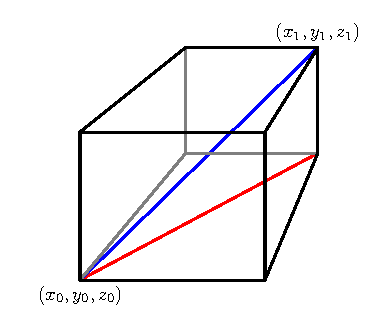
\includegraphics{figures/fig_9_1_distance.eps}
\caption{The distance formula in $\R^3$.}
\label{F:9.1.Distance_3D}
\end{center}
\end{figure}
    \ba
  \item Consider one of the right triangles in the base of the box whose
    hypotenuse is shown as the red line in Figure
    \ref{F:9.1.Distance_3D}. What are the vertices of this triangle?
    Since this right triangle lies in a plane, we can use the
    Pythagorean Theorem to find a formula for the length of the
    hypotenuse of this triangle. Find such a formula, which will be in
    terms of $x_0$, $y_0$, $x_1$, and $y_1$.

  \item Now notice that the triangle whose hypotenuse is the blue segment
    connecting the points $P$ and $Q$ with a leg as the hypotenuse of
    the triangle found in part (a) lies entirely in a plane, so we can
    again use the Pythagorean Theorem to find the length of its
    hypotenuse. Explain why the length of this hypotenuse, which is
    the distance between the points $P$ and $Q$, is
        \begin{equation*} %\label{eq:9.1.Distance_3D}
        \sqrt{(x_1-x_0)^2 + (y_1-y_0)^2 + (z_1-z_0)^2}.
        \end{equation*}

    \ea
\end{activity}
\begin{smallhint}
\ba
\item What are the equations of the faces of the box?
\item What is the distance between the point $Q$ and the point at the lower right corner of the back of the box? 
\ea

\end{smallhint}
\begin{bighint}
\ba
\item The front face of the box has equation $x=x_0$ and the right face of the box has equation $y=y_1$. 
\item What is the distance between the point $Q$ and the point at the lower right corner of the back of the box? 
\ea
\end{bighint}
\begin{activitySolution}
\ba
\item The front face of the box is the $x=x_0$ plane, the back is the $x=x_1$ plane, the bottom is the $z=z_0$ plane, and the right side is the $y=y_1$ plane. So the coordinates of the point at the lower front right of the box are $(x_0,y_1,z_0)$ and the coordinates of the point at the back lower right of the box are $(x_1, y_1, z_0)$. The length of the legs of this triangle are $\mid y_1-y_0\mid$  (the distance between the points $(x_0, y_0, z_0)$ and $(x_0,y_1,z_0)$) and $\mid x_1-x_0 \mid$ (the distance between the points $(x_0, y_1, z_0)$ and $(x_1,y_1,z_0)$). The Pythagorean Theorem then shows that the length of the hypotenuse of the triangle in the base of the box is  
\[\sqrt{(x_1-x_0)^2+(y_1-y_0)^2}.\]
\item The distance between $P$ and $Q$ is the length of the hypotenuse of the triangle whose legs are the hypotenuse of the triangle in the base of the box and whose height is the distance between the points $Q=(x_1,y_1,z_1)$ and $R=(x_1, y_1, z_0)$ (the point at the bottom right corner of the back of the box). The distance between $Q$ and $R$ is just $\mid z_1-z_0\mid$. Using the result from part (a), the Pythagorean Theorem shows that the distance between $P$ and $Q$ is 
\[\sqrt{\left(\sqrt{(x_1-x_0)^2+(y_1-y_0)^2}\right)^2 + (z_1-z_0)^2} = \sqrt{(x_1-x_0)^2 + (y_1-y_0)^2 + (z_1-z_0)^2}\]
as desired.  
\ea
\end{activitySolution}
\aftera 


The formula developed in Activity \ref{A:9.1.4} is important to remember.

\vspace*{5pt}
\nin \framebox{\hspace*{3 pt}
\parbox{6.25 in}{The distance between points $P=(x_0, y_0, z_0)$ and $Q=(x_1, y_1, z_1)$ (denoted as $|PQ|$)  in $\R^3$ is given by the formula
\begin{equation} \label{eq:9.1.Distance_3D}
|PQ| = \sqrt{(x_1-x_0)^2 + (y_1-y_0)^2 + (z_1-z_0)^2}.
\end{equation}
} \hspace*{3 pt}}
\vspace*{5pt}

Equation (\ref{eq:9.1.Distance_3D}) can be used to derive the formula
for a sphere\index{sphere!formula} centered at a point $(x_0,y_0,z_0)$
with radius $r$. Since the distance from any point $(x,y,z)$ on such a
sphere to the point $(x_0,y_0,z_0)$ is $r$, the point $(x,y,z)$ will
satisfy the equation
\[\sqrt{(x-x_0)^2 + (y-y_0)^2 + (z-z_0)^2} = r\]
%or
%\[(x-x_0)^2 + (y-y_0)^2 + (z-z_0)^2 = r^2.\]
Squaring both sides, we come to the standard equation for a sphere.

\vspace*{5pt}
\nin \framebox{\hspace*{3 pt}
\parbox{6.25 in}{The equation of a sphere with center $(x_0,y_0,z_0)$ and radius $r$ is
\[(x-x_0)^2 + (y-y_0)^2 + (z-z_0)^2 = r^2.\]
} \hspace*{3 pt}}
\vspace*{5pt}

This makes sense if we compare this equation to its two-dimensional
analogue, the equation of a circle of radius $r$ in the plane centered
at $(x_0,y_0)$:
$$
(x-x_0)^2 + (y-y_0)^2 = r^2.
$$


%\begin{activity} \label{A:9.1.5}
    Find the equation of the sphere centered at the point $(2,1,3)$ if the point $(-1,0,-1)$ lies on the sphere.

\end{activity}
\begin{smallhint}

\end{smallhint}
\begin{bighint}

\end{bighint}
\begin{activitySolution}

\end{activitySolution}
\aftera 

\subsection*{Traces}

When we study functions of several variables we are often interested
in how each individual variable affects the function in and of
itself. In Preview Activity \ref{PA:9.1}, we saw that the monthly
payment on an \$18,000 loan depends on the interest rate and the
duration of the loan. However, if we fix the interest rate, the
monthly payment depends only on the duration of the loan, and if we
set the duration the payment depends only on the interest rate. This
idea of keeping one variable constant while we allow the other to
change will be an important tool for us when studying functions of
several variables.

As another example, consider again the range function $f$ defined by
\[f(x,y) = \frac{x^2 \sin(2y)}{g}\] where $x$ is the initial velocity
of an object in feet per second, $y$ is the launch angle in radians,
and $g$ is the acceleration due to gravity (32 feet per second
squared). If we hold the launch angle constant at $y=0.6$ radians, we
can consider $f$ a function of the initial velocity alone. In this
case we have
\[f(x) = \frac{x^2}{32}\sin(2\cdot 0.6).\]
We can plot this curve on the surface by tracing out the points on the
surface when $y = 0.6$, as shown in Figure
\ref{F:9.1.trace1}. The graph and the formula clearly show that $f$ is
quadratic in the $x$-direction. More descriptively, as we increase the
launch velocity while keeping the launch angle constant, the range
increases proportional to the square of the initial velocity.

Similarly, if we fix the initial velocity at 150 feet per second, we
can consider the range as a function of the launch angle only. In this
case we have
\[f(y) = \frac{150^2 \sin(2y)}{32}.\] 
We can again plot this curve on
the surface by tracing out the points on the surface when $x=150$, as
shown in Figure \ref{F:9.1.trace2}. The graph and the formula clearly
show that $f$ is sinusoidal in the $y$-direction. More descriptively,
as we increase the launch angle while keeping the initial velocity
constant, the range is proportional to the sine of twice the launch
angle.
\begin{figure}[ht]
\begin{center}
\begin{minipage}{2.5in}
\begin{center}
%\resizebox{!}{1.75in}{\includegraphics[trim=0cm 0cm 1cm 4.5cm,
%clip]{9_1_trace1}}
  \includegraphics{figures/fig_9_1_y_range.eps}
\caption{The trace with $y = 0.6$.}
\label{F:9.1.trace1}
\end{center}
\end{minipage}
\hspace{0.5in}
\begin{minipage}{2.5in}
\begin{center}
%\resizebox{!}{1.75in}{\includegraphics[trim=0cm 0cm 1cm 4.5cm, clip]{9_1_trace2}}
  \includegraphics{figures/fig_9_1_x_range.eps}
\caption{The trace with $x = 150$.}
\label{F:9.1.trace2}
\end{center}
\end{minipage}
\end{center}
\end{figure}

The curves we define when we fix one of the independent variables in our two variable function are called \emph{traces}.

\vspace*{5pt}
\nin \framebox{\hspace*{3 pt}
\parbox{6.25 in}{\begin{definition} A \textbf{trace}\index{trace} of a function $f$ of two independent variables $x$ and $y$ is a curve of the form $z = f(c,y)$ or $z = f(x,c)$, where $c$ is a constant. \end{definition}
} \hspace*{3 pt}}
\vspace*{5pt}

Understanding trends in the behavior of functions of two variables can
be challenging, as can sketching their graphs; traces help us with
each of these tasks.

\begin{activity} \label{A:9.1.6}
    In the following questions, we investigate the use of traces to better understand a function through both tables and graphs.  
    \ba
  \item Identify the $y = 0.6$ trace for the range function $f(x,y) =
    \frac{x^2 \sin(2y)}{g}$ by highlighting or circling the
    appropriate cells in Table \ref{T:9.1.range}.  Write a sentence to
    describe the behavior of the function along this trace.

  \item Identify the $x = 150$ trace for the range function by
    highlighting or circling the appropriate cells in Table
    \ref{T:9.1.range}.  Write a sentence to describe the behavior of
    the function along this trace.

 \begin{figure}[ht]
\begin{center}
%\resizebox{!}{2.0in}{\includegraphics{figures/9_1_traces_activity_1}}
  \includegraphics{figures/fig_9_1_activity_axes.eps}
\caption{Coordinate axes to sketch traces.}
\label{F:9.1.traces_activity_1}
\end{center}
\end{figure}

   \item For the function $g(x,y) = x^2 + y^2 + 1$, explain the type of function that each trace in the $x$ direction will be (keeping $y$ constant). Plot the $y=-4$, $y=-2$, $y=0$, $y=2$, and $y=4$ traces in 3-dimensional coordinate system provided in Figure \ref{F:9.1.traces_activity_1}.

    \item For the function $g(x,y) = x^2 + y^2 + 1$, explain the type of function that each trace in the $y$ direction will be (keeping $x$ constant). Plot the $x=-4$, $x=-2$, $x=0$, $x=2$, and $x=4$ traces in 3-dimensional coordinate system in Figure \ref{F:9.1.traces_activity_1}.

    \item Describe the surface generated by the function $g$.

     \ea



\end{activity}
\begin{smallhint}
\ba
\item Do the $y$ values run down the columns or across the rows?
\item Do the $x$ values run down the columns or across the rows?
\item If $y$ is constant, the only variables are $x$ and $z$. 
\item If $x$ is constant, the only variables are $y$ and $z$.
\item What do the traces look like?
\ea 
\end{smallhint}
\begin{bighint}
\ba
\item Do the $y$ values run down the columns or across the rows?
\item Do the $x$ values run down the columns or across the rows?
\item What does the graph of $z=x^2+C$ look like if $C$ is a constant?
\item What does the graph of $z=y^2+C$ look like if $C$ is a constant?
\item What do the traces look like?
\ea
\end{bighint}
\begin{activitySolution}
\ba
\item The $y$ values in the table are those that run across the rows. So fixing $y$ at $\frac{2\pi}{5} = \frac{8\pi}{20}$ and letting $x$ vary amounts to looking at the $\frac{8\pi}{20}$ column in the table. The $y=\frac{2\pi}{5}$ trace is highlighted in red in the table below. This trace shows that as we increase the initial velocity $x$ while keeping the launch angle constant at $\frac{2\pi}{5}$ radians, the range of the object increases at an increasing rate. 
\begin{center}
\begin{tabular}{|c|c|c|c|c|c|c|c|>{\columncolor{tracered}}c|c|c|} \hline
  &$\frac{\pi}{20}$ &$\frac{2\pi}{20}$ &$\frac{3\pi}{20}$ &$\frac{4\pi}{20}$ &$\frac{5\pi}{20}$ &$\frac{6\pi}{20}$ &$\frac{7\pi}{20}$ &$\frac{8\pi}{20}$ &$\frac{9\pi}{20}$    &$\frac{\pi}{2}$ \\ \hline
25      &6.036      &11.480     &15.801     &18.575     &19.531     &18.575     &15.801     &11.480     &6.0356     &0.000 \\ \hline
50      &24.142     &45.921     &63.205     &74.301     &78.125     &74.301     &63.205     &45.921     &24.142     &0.000 \\ \hline
75      &54.319     &103.322    &142.210    &167.178    &175.781    &167.178    &142.210    &103.322    &54.319     &0.000 \\ \hline
100     &96.568     &183.683    &252.818    &297.205    &312.500    &297.205    &252.818    &183.683    &96.568     &0.000 \\ \hline
125     &150.887    &287.005    &395.028    &464.383    &488.281    &464.383    &395.028    &287.005    &150.887    &0.000 \\ \hline
150     &217.278    &413.287    &568.840    &668.712    &703.125    &668.712    &568.840    &413.287    &217.278    &0.000 \\ \hline
175     &295.739    &562.529    &774.255    &910.191    &957.031    &910.191    &774.255    &562.529    &295.739    &0.000 \\ \hline
200     &386.271    &734.732    &1011.271   &1188.821   &1250.000   &1188.821   &1011.271   &734.732    &386.271    &0.000 \\ \hline
225     &488.875    &929.895    &1279.890   &1504.601   &1582.031   &1504.601   &1279.890   &929.895    &488.875    &0.000 \\ \hline
250     &603.549    &1148.018   &1580.112   &1857.532   &1953.125   &1857.532   &1580.112   &1148.018   &603.549    &0.000 \\ \hline
\end{tabular}
\end{center}
\item  The $x$ values in the table are those that run down the columns. So fixing $x$ at $150$ and letting $y$ vary amounts to looking at the $150$ row in the table. The $x=150$ trace is highlighted in blue in the table below. This trace shows that as we increase the launch angle $y$ while keeping the initial velocity $x$ at a constant $150$ feet per second, the range increases at first until we reach an angle of approximately $\frac{pi}{4}$, and then decreases. 
%\begin{table}[ht]
\begin{center}
\begin{tabular}{|c|c|c|c|c|c|c|c|c|c|c|} \hline
  &$\frac{\pi}{20}$ &$\frac{2\pi}{10}$ &$\frac{3\pi}{20}$ &$\frac{4\pi}{20}$ &$\frac{5\pi}{20}$ &$\frac{6\pi}{20}$ &$\frac{7\pi}{20}$ &$\frac{8\pi}{20}$ &$\frac{9\pi}{20}$    &$\frac{\pi}{2}$ \\ \hline
25      &6.036      &11.480     &15.801     &18.575     &19.531     &18.575     &15.801     &11.480     &6.0356     &0.000 \\ \hline
50      &24.142     &45.921     &63.205     &74.301     &78.125     &74.301     &63.205     &45.921     &24.142     &0.000 \\ \hline
75      &54.319     &103.322    &142.210    &167.178    &175.781    &167.178    &142.210    &103.322    &54.319     &0.000 \\ \hline
100     &96.568     &183.683    &252.818    &297.205    &312.500    &297.205    &252.818    &183.683    &96.568     &0.000 \\ \hline
125     &150.887    &287.005    &395.028    &464.383    &488.281    &464.383    &395.028    &287.005    &150.887    &0.000 \\ \hline
150     &217.278    &413.287    &568.840    &668.712    &703.125    &668.712    &568.840    &413.287    &217.278    &0.000 \\ \hline
175     &295.739    &562.529    &774.255    &910.191    &957.031    &910.191    &774.255    &562.529    &295.739    &0.000 \\ \hline
\rowcolor{traceblue}
200     &386.271    &734.732    &1011.271   &1188.821   &1250.000   &1188.821   &1011.271   &734.732    &386.271    &0.000 \\ \hline
225     &488.875    &929.895    &1279.890   &1504.601   &1582.031   &1504.601   &1279.890   &929.895    &488.875    &0.000 \\ \hline
250     &603.549    &1148.018   &1580.112   &1857.532   &1953.125   &1857.532   &1580.112   &1148.018   &603.549    &0.000 \\ \hline
\end{tabular}
%\caption{Values of $f(x,y) = \frac{x^2 \sin(2y)}{g}$.}
%\label{T:tracey_sol}
\end{center}
%\end{table}
\item The portion of the surface $g$ where $y$ is constant at a value $k$ has the form 
\[g(x,k) = x^2+k^2+1.\]
This is a quadratic parallel to the $xz$-plane with its vertex at the point $(0,k,k^2+1)$, opening in the positive $z$ direction. The indicated traces are shown here %in Figure \ref{F:9.1_Act_6_1}
%\begin{figure}[ht]
\begin{center}
\resizebox{!}{2.0in}{\includegraphics{figures/9_1_Act_6_1}}
%\caption{Traces in the $x$ direction.}
%\label{F:9.1_Act_6_1}
\end{center}
%\end{figure}
 \item The portion of the surface $g$ where $x$ is constant at a value $c$ has the form 
\[g(c,y) = c^2+y^2+1.\]
This is a quadratic parallel to the $yz$-plane with its vertex at the point $(c,0,c^2+1)$, opening in the positive $z$ direction. The indicated traces are shown here %in Figure \ref{F:9.1_Act_6_2}
%\begin{figure}[ht]
\begin{center}
\resizebox{!}{2.0in}{\includegraphics{figures/9_1_Act_6_2}}
%\caption{Traces in the $y$ direction.}
%\label{F:9.1_Act_6_2}
\end{center}
%\end{figure}
\item The traces of $g$ in both directions are parabolas opening in the positive $z$ direction. So the graph of $g$ should look like a bowl with its vertex at the origin, opening in the positive $z$ direction. 
\ea
\end{activitySolution}
\aftera 

%\input{activities/9.1.Act7}

\subsection*{Contour Maps and Level Curves}

We have all seen topographic maps such as the one of the Porcupine
Mountains in the upper peninsula of Michigan shown in Figure
\ref{F:9.1.porcupine}.\footnote{Map source: Michigan Department of
  Natural Resources,
  \url{https://www.michigan.gov/dnr/0,4570,7-153-10369_46675_58093---,00.html},
  with permission of the Michigan DNR and Bob Wild.} The curves on
these maps show the regions of constant altitude. The contours also
depict changes in altitude: contours that are close together signify
steep ascents or descents, while contours that are far apart indicate
only slight changes in elevation.  Thus, contour maps tell us a lot
about three-dimensional surfaces. Mathematically, if $f(x,y)$
represents the altitude at the point $(x,y)$, then each contour is the
graph of an equation of the form $f(x,y) = k$, for some constant $k$.

\newpage
\begin{landscape}
\begin{figure}[h]
\begin{center}
\resizebox{!}{5.0in}
{\includegraphics[trim=55cm 40cm 40cm 40cm, clip]{9_1_porcupine_2}}
%trim=left bottom right top, need clip if not animation
% 
\caption{Contour map of the Porcupine Mountains.}
\label{F:9.1.porcupine}
\end{center}
\end{figure}
\end{landscape}
\newpage

\begin{activity} \label{A:9.1.8}
   On the topographical map of the Porcupine Mountains in Figure \ref{F:9.1.porcupine},

   \ba
    \item identify the highest and lowest points you can find;
    \item from a point of your choice, determine a path of steepest ascent that leads to the highest point;
    \item from that same initial point, determine the least steep path that leads to the highest point.

     \ea

\end{activity}
\begin{smallhint}

\end{smallhint}
\begin{bighint}
\ba
\item The best you can do is search the map for the highest and lowest elevations.
\item Closely spaced contours indicate a sharp increase or decrease in elevation.
\item Widely spaced contours indicate a slow increase or decrease in elevation. 
\ea
\end{bighint}
\begin{activitySolution}
\ba
\item Summit Peak appears to be the highest point on this map at an elevation of around 593. Near the top left corner of the map there is a contour at an elevation of around 200 that seems to be the lowest on the map. 
\item The contours to the west of Summit Peak appear to be the most closely spaced, indicating the path of steepest ascent to the peak.
\item The contours to the southwest of Summit Peak appear to be the most widely spaced, indicating the path of most gentle ascent to the peak.
\ea
\end{activitySolution}

%\newpage
%\begin{landscape}
%\begin{figure}[ht]
%\begin{center}
%\resizebox{!}{4.0in}{\includegraphics[trim=40cm 40cm 40cm 40cm, clip]{figures/1_1_porcupine_2}} %trim=left bottom right top, need clip if not animation
%\caption{Contour map of the Porcupine Mountains.}
%\label{F:1.1.porcupine}
%\end{center}
%\end{figure}
%\end{landscape}
%\newpage

\aftera 

\vspace*{5pt}
\nin \framebox{\hspace*{3 pt}
\parbox{6.25 in}{\begin{definition} A \textbf{level curve\index{level curve} (or contour)} of a function $f$ of two independent variables $x$ and $y$ is a curve of the form $k = f(x,y)$, where $k$ is a constant. \end{definition}
} \hspace*{3 pt}}
\vspace*{5pt}

Topographical maps can be used to create a three-dimensional surface
from the two-dimensional contours or level curves. For example, level
curves of the range function, $f(x,y) = \frac{x^2 \sin(2y)}{32}$,
plotted in the $xy$-plane are shown in Figure
\ref{F:9.1.contours_1}. If we lift these contours and plot them at
their respective heights, then we get a picture of the surface itself,
as illustrated in Figure \ref{F:9.1.contours_2}.

\begin{figure}[ht]
\begin{center}
\begin{minipage}{2.5in}
\begin{center}
%\resizebox{!}{1.75in}{\includegraphics{9_1_contours1}}
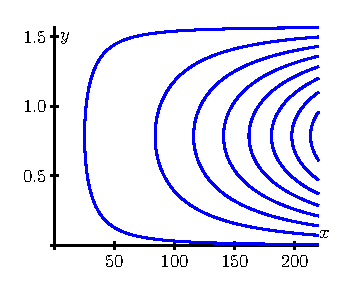
\includegraphics{figures/fig_9_1_contour_1.eps}
\caption{Several level curves.}
\label{F:9.1.contours_1}
\end{center}
\end{minipage}
\hspace{0.5in}
\begin{minipage}{2.5in}
\begin{center}
%\resizebox{!}{1.75in}{\includegraphics[trim=0cm 0cm 1cm 4.5cm, clip]{9_1_contours2}}
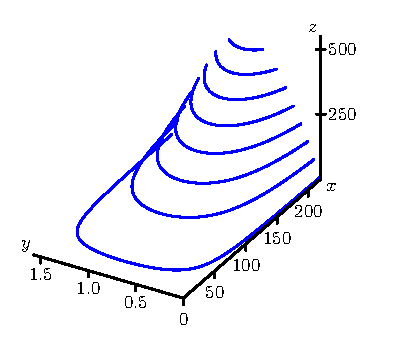
\includegraphics{figures/fig_9_1_contour_2.eps}
\caption{Level curves at the appropriate height.}
\label{F:9.1.contours_2}
\end{center}
\end{minipage}
\end{center}
\end{figure}

The use of level curves and traces can help us construct the graph of
a function of two variables.


\begin{activity} \label{A:9.1.9}
\begin{figure}[ht]
\begin{center}
%\resizebox{!}{1.75in}{\includegraphics{figures/9_1_contour_activity_1}} 
%\hspace{0.2in} 
%\resizebox{!}{1.75in}{\includegraphics{figures/9_1_contour_activity_1}}
  \includegraphics{figures/fig_9_1_activity_empty_1.eps}
  \hspace*{0.5in}
  \includegraphics{figures/fig_9_1_activity_empty_2.eps}
\caption{Left: Level curves for $f(x,y) = x^2+y^2$. Right: Level curves for $g(x,y) = \sqrt{x^2+y^2}$.}
\label{F:9.1.contour_activity}
\end{center}
\end{figure}
   \ba
    \item Let $f(x,y) = x^2+y^2$. Draw the level curves $f(x,y) = k$ for $k=1$, $k=2$, $k=3$, and $k=4$ on the left set of axes given in Figure \ref{F:9.1.contour_activity}. (You decide on the scale of the axes.) Explain what the surface defined by $f$ looks like.

    \item Let $g(x,y) = \sqrt{x^2+y^2}$. Draw the level curves $g(x,y) = k$ for $k=1$, $k=2$, $k=3$, and $k=4$ on the right set of axes given in Figure \ref{F:9.1.contour_activity}. (You decide on the scale of the axes.) Explain what the surface defined by $g$ looks like.

    \item Compare and contrast the graphs of $f$ and $g$. How are they alike? How are they different? Use traces for each function to help answer these questions.

     \ea

\end{activity}
\begin{smallhint}
\ba
\item The contours have graphs that should be familiar. 
\item The contours have graphs that should be familiar.
\item How well spaced are the contours of $f$ and $g$?  
\ea
\end{smallhint}
\begin{bighint}
\ba
\item What familiar graph does the equation $x^2+y^2=1$ have?
\item What equation do you get if you square both sides of $1 = \sqrt{x^2+y^2}$?
\item What kind of graph is $y=x^2+C$ where $C$ is a constant? What kind of graph if $y = \sqrt{x^2}$? 
\ea
\end{bighint}
\begin{activitySolution}
\ba
\item The contours of $f$ are shown at left in the figure below.  The contours are circles, getting closer together as we move away from the origin, indicating a graph that is increasing quickly as we move away from the origin in all directions. The surface defined by $f$ looks like a bowl anchored at the origin that opens up. %Figure \ref{F:9.1.contour_activity_sol}.
\item The contours of $g$ are shown at right in the figure below. The contours are circles that appear to be uniformly spaced as we move away from the origin. This indicates that the surface defined by $g$ looks like a cone anchored at the origin that opens up. %Figure \ref{F:9.1.contour_activity_sol}. 
    \item The contours of $g$ are more uniformly spaced as we move away from the origin than those  in part (a). So we should expect the graph of $f$ to increase more rapidly as we move radially from the origin than the graph of $g$. To see this in another light, the traces of $f$ for fixed $y$ have the form $z = k^2+x^2$ for constants $k$, which are parabolic in form. By symmetry, the traces of $f$ for fixed values of $x$ have the same shape. By contrast, the traces of $g$ for fixed $y$ have the form $z = \sqrt{k^2+x^2}$ for constants $k$. In particular, the trace with $k=0$ has the form $z = \sqrt{x^2} = | x |$, which is linear. By symmetry, the traces for fixed $y$ have the same shape. This confirms our statements in (a) and (b) that the graph of $f$ is parabolic (bowl shaped), while the graph of $g$ looks like a cone. 
    \ea
%\begin{figure}[ht]
\begin{center}
\resizebox{!}{1.75in}{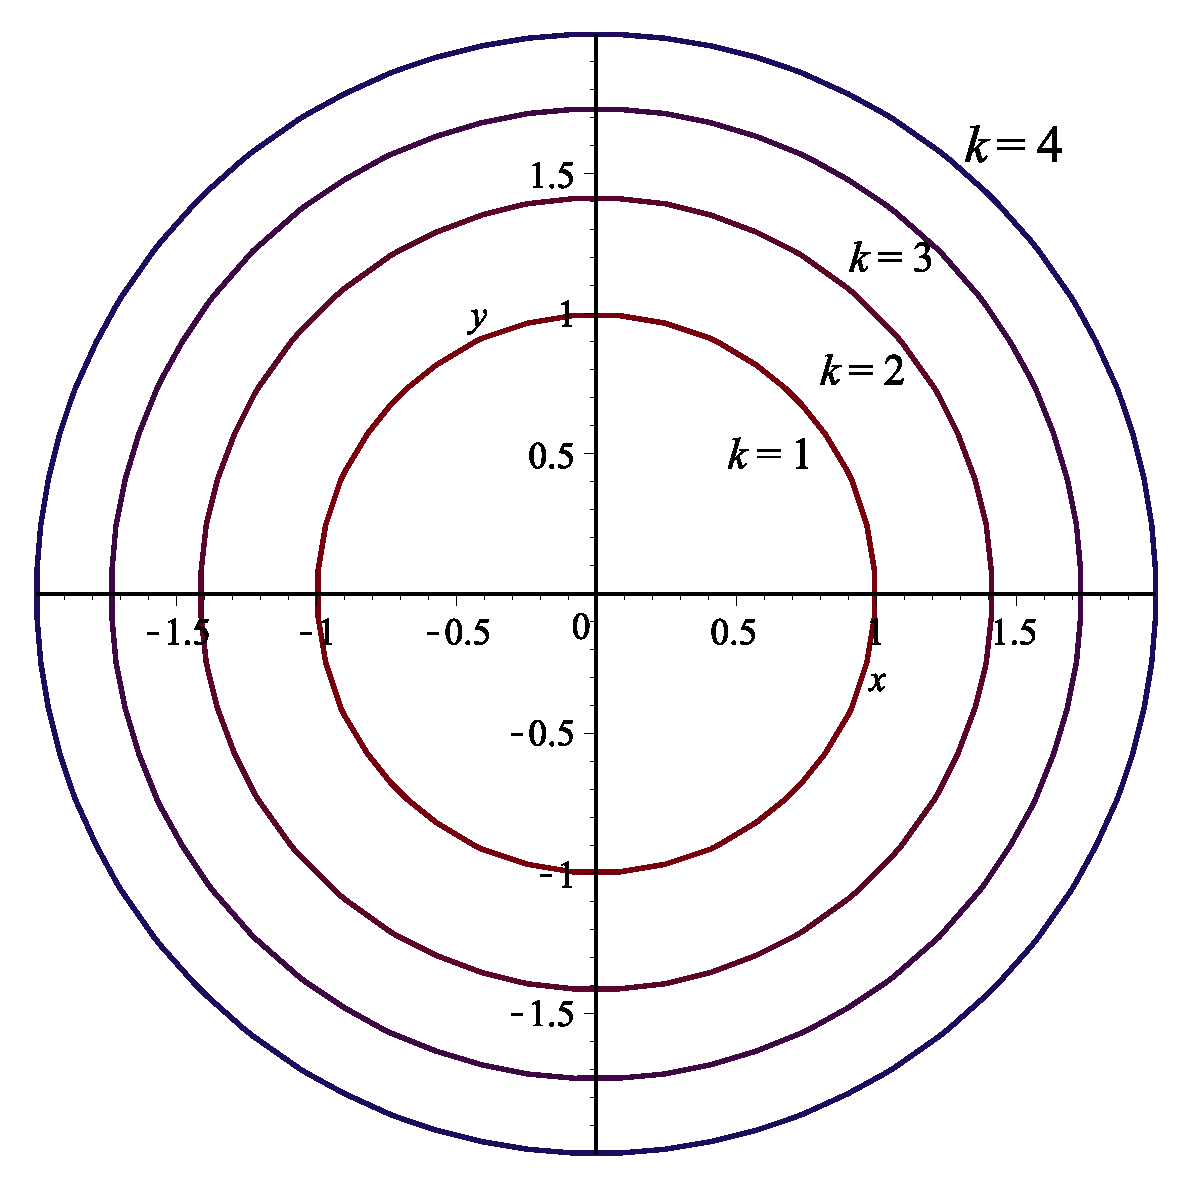
\includegraphics{figures/9_1_contour_activity_1a}} \hspace{0.2in} \resizebox{!}{1.75in}{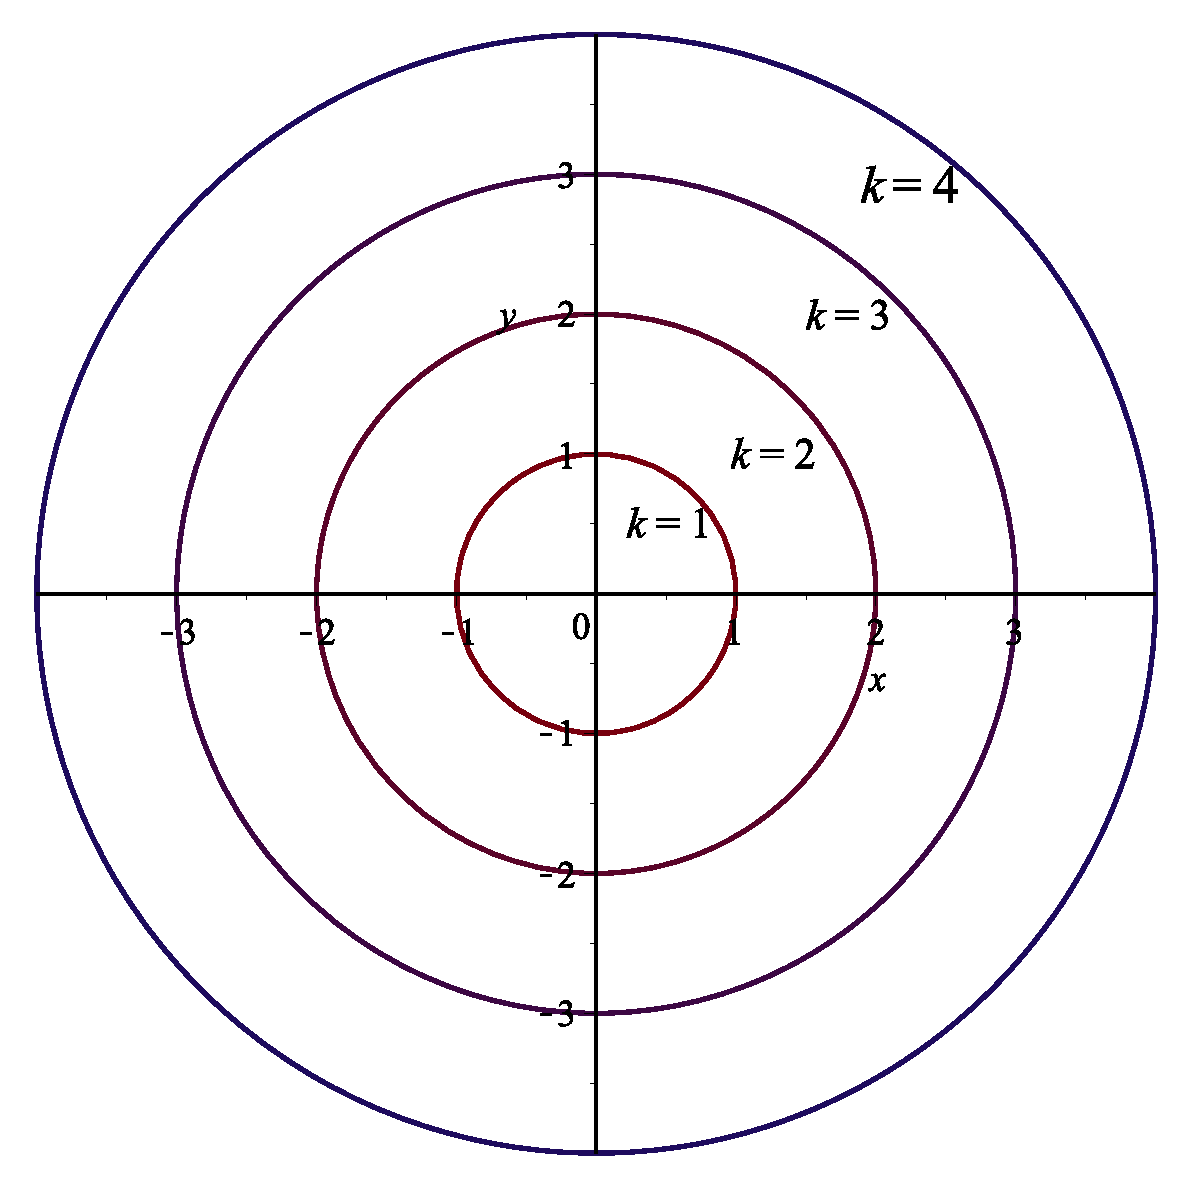
\includegraphics{figures/9_1_contour_activity_1b}}
%\caption{Left:Level curves for $f(x,y) = x^2+y^2$. Right: Level curves for $g(x,y) = \sqrt{x^2+y^2}$.}
%\label{F:9.1.contour_activity_sol}
\end{center}
%\end{figure}
\end{activitySolution}


\aftera 

%
\begin{activity} \label{A:9.1.10}
The Ideal Gas Law $PV = RT$ relates the pressure ($P$, in pascals), temperature ($T$, in Kelvin), and volume ($V$, in cubic meters) of 1 mole of a gas ($R =  8.314 \ \frac{\text{J}}{\text{mol} \ \text{K}}$ is the universal gas constant), and describes the behavior of gases that do not liquefy easily, such as oxygen and hydrogen. We can solve the ideal gas law for the volume and treat the volume as a function of the pressure and temperature:
\[V(P,T) = \frac{8.314T}{P}.\]
    \ba
    \item Explain in detail what the trace of $V$ with $P=1000$ tells us.
    \item Explain in detail what the trace of $V$ with $T=5$ tells us.
    \item Explain in detail what the level curve $V = 0.5$ tells us.
    \ea
\end{activity}
\begin{smallhint}

\end{smallhint}
\begin{bighint}

\end{bighint}
\begin{activitySolution}


\end{activitySolution}


\aftera 

The traces and level curves of a function of two variables are curves
in space. In order to understand these traces and level curves better,
we will first spend some time learning about vectors and vector-valued
functions in the next few sections and return to our study of
functions of several variables once we have those more mathematical
tools to support their study.

\subsection*{A gallery of functions}

We end this section by considering a collection of functions and
illustrating their graphs and some level curves.

\begin{figure}[ht]
  \begin{center}
    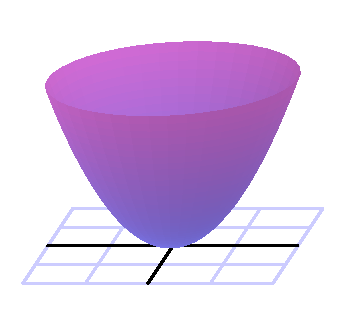
\includegraphics{figures/zisr2.eps}
    \hspace*{30pt}
    \includegraphics{figures/zisr2_contours.eps}
  \end{center}
  \caption{$z=x^2+y^2$}
\end{figure}
\begin{figure}[ht]
  \begin{center}
    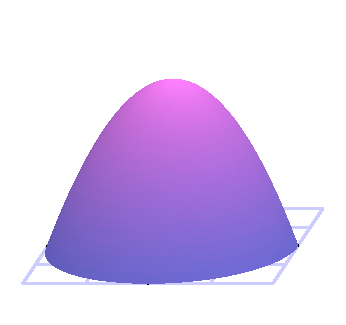
\includegraphics{figures/zis4r2.eps}
    \hspace*{30pt}
    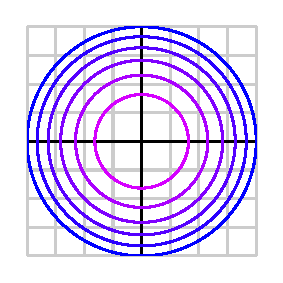
\includegraphics{figures/zis4r2_contours.eps}
  \end{center}
  \caption{$z=4-(x^2+y^2)$}
\end{figure}
\begin{figure}[ht]
  \begin{center}
    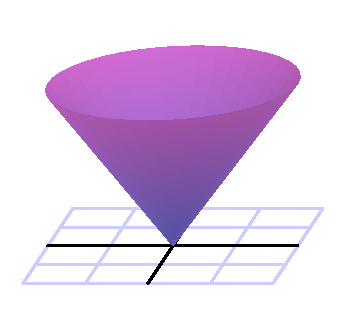
\includegraphics{figures/cone.eps}
    \hspace*{30pt}
    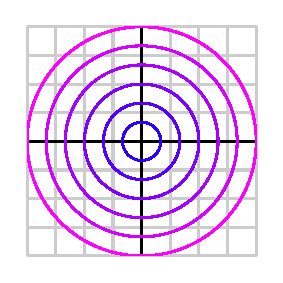
\includegraphics{figures/cone_contours.eps}
  \end{center}
  \caption{$z=\sqrt{x^2+y^2}$}
\end{figure}
\clearpage
\begin{figure}[ht]
  \begin{center}
    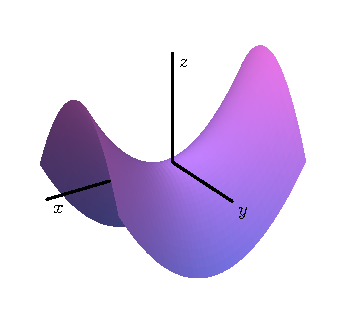
\includegraphics{figures/saddle.eps}
    \hspace*{30pt}
    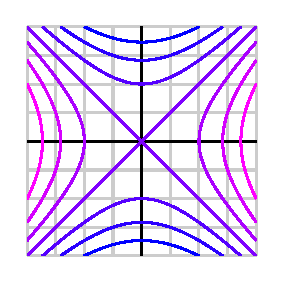
\includegraphics{figures/saddle_contours.eps}
  \end{center}
  \caption{$z=x^2-y^2$}
\end{figure}
\begin{figure}[ht]
  \begin{center}
    
\includegraphics{figures/sinxy.eps}
    \hspace*{30pt}
    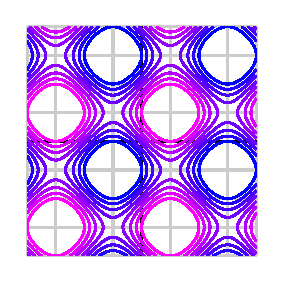
\includegraphics{figures/sinxy_contours.eps}
  \end{center}
  \caption{$z=\sin(x)+\sin(y)$}
\end{figure}
\clearpage
\begin{figure}[ht]
  \begin{center}
    
\includegraphics{figures/elliptic.eps}
    \hspace*{30pt}
    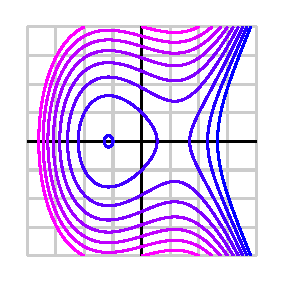
\includegraphics{figures/elliptic_contours.eps}
  \end{center}
  \caption{$z=y^2 - x^3 + x$}
\end{figure}
\begin{figure}[ht]
  \begin{center}
    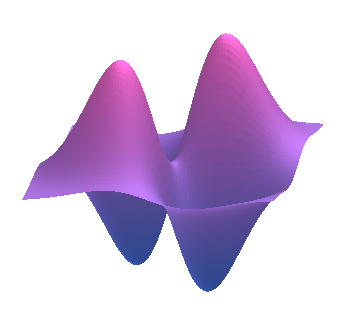
\includegraphics{figures/exp.eps}
    \hspace*{30pt}
    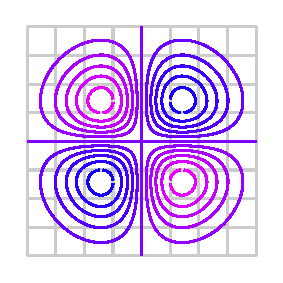
\includegraphics{figures/exp_contours.eps}
  \end{center}
  \caption{$z=xye^{-x^2-y^2}$}
\end{figure}


%\nin \framebox{\hspace*{3 pt}
%\parbox{6.25 in}{
\begin{summary}
%\item A three-dimensional system has two possible orientations. In a right hand system, if we point the index finger of our right hand in the direction of the positive $x$-axis and our middle finger in the direction of the positive $y$-axis, then our thumb will point in the direction of the positive $z$-axis. A left hand system has a different orientation and we need pick one as a standard so that the convention of orientation is understood by everyone.
\item A function $f$ of several variables is a rule that assigns a unique number to an ordered collection of independent inputs.  The domain of a function of several variables is the set of all inputs for which the function is defined.
\item In $\R^3$, the distance between points $P=(x_0, y_0, z_0)$ and $Q=(x_1, y_1, z_1)$ (denoted as $|PQ|$)  is given by the formula
\[|PQ| = \sqrt{(x_1-x_0)^2 + (y_1-y_0)^2 + (z_1-z_0)^2}.\]
and thus the equation of a sphere with center $(x_0,y_0,z_0)$ and radius $r$ is
\[(x-x_0)^2 + (y-y_0)^2 + (z-z_0)^2 = r^2.\]
\item A trace of a function $f$ of two independent variables $x$ and $y$ is a curve of the form $z = f(c,y)$ or $z = f(x,c)$, where $c$ is a constant. A trace tells us how the function depends on a single independent variable if we treat the other independent variable as a constant. 
\item A level curve of a function $f$ of two independent variables $x$ and $y$ is a curve of the form $k = f(x,y)$, where $k$ is a constant. A level curve describes the set of inputs that lead to a specific output of the function.
\end{summary}
%} \hspace*{3 pt}}

\nin \hrulefill

\begin{exercises} 

\item \label{Ez:9.1.1}   Find the equation of each of the following geometric objects.

%\begin{figure}[h]
%\begin{center}
 %\includegraphics{figures/1_1_Ez1.eps}
 %\caption{A bungee jumper's height function.} \label{F:1.1.Ez1}
%\end{center}
%\end{figure}

  \ba
  	\item  The plane parallel to the $x$-$y$ plane that passes through the point $(-4,5,-12)$.
	\item  The plane parallel to the $y$-$z$ plane that passes through the point $(7, -2, -3)$.
	\item   The sphere centered at the point $(2,1,3)$ and has the point $(-1,0,-1)$ on its surface.
	\item  The sphere whose diameter has endpoints $(-3,1,-5)$ and $(7,9,-1)$.
  
  \ea 

\begin{exerciseSolution}
  \ba
  	\item  A plane parallel to the $x$-$y$ plane has constant $z$-coordinate. So the equation of the plane parallel to the $x$-$y$ plane that passes through the point $(-4,5,-12)$ is $z=-12$. 
	\item   A plane parallel to the $y$-$z$ plane has constant $x$-coordinate. So the equation of the plane parallel to the $y$-$z$ plane that passes through the point $(7, -2, -3)$ is $x=7$.
	\item   The radius of the sphere is the distance from the center $(2,1,3)$ to the point $(-1,0,-1)$, so the radius of this sphere is $\sqrt{(2-(-1))^2 + (1-0)^2 + (3-(-1))^2} = \sqrt{26}$. So the equation of this sphere is $(x-2)^2 + (y-1)^2 + (z-3)^2 = 26$. 
	\item  The center of the sphere will be the midpoint of the segment connecting the endpoints $(-3,1,-5)$ and $(7,9,-1)$. This midpoint is $\left(\frac{-3+7}{2}, \frac{1+9}{2}, \frac{-5+(-1)}{2} \right) = (2, 5, -3)$. The radius of the sphere is the distance from its center to either endpoint of the segment or $\sqrt{(2-(-1))^2 + (5-1)^2 + (-3-(-5))^2} = \sqrt{29}$. So the equation of this sphere is $(x-2)^2 + (y-5)^2 + (z+3)^2 = 29$.
  
  \ea 
\end{exerciseSolution}


\item \label{Ez:9.1.2}   The Ideal Gas Law, $PV = RT$, relates the pressure ($P$, in pascals), temperature ($T$, in Kelvin), and volume ($V$, in cubic meters) of 1 mole of a gas ($R =  8.314 \ \frac{\text{J}}{\text{mol} \ \text{K}}$ is the universal gas constant), and describes the behavior of gases that do not liquefy easily, such as oxygen and hydrogen. We can solve the ideal gas law for the volume and hence treat the volume as a function of the pressure and temperature:
\[V(P,T) = \frac{8.314T}{P}.\]
    \ba
    \item Explain in detail what the trace of $V$ with $P=1000$ tells us about a key relationship between two quantities.
    \item Explain in detail what the trace of $V$ with $T=5$ tells us.
    \item Explain in detail what the level curve $V = 0.5$ tells us.
    \item Use 2 or three additional traces in each direction to make a rough sketch of the surface over the domain of $V$ where $P$ and $T$ are each nonnegative.  Write at least one sentence that describes the way the surface looks.
    \item Based on all your work above, write a couple of sentences that describe the effects that temperature and pressure have on volume.
    \ea
    
\begin{exerciseSolution}
    \ba
    \item The $P=1000$ trace tells us the volume of 1 mole of a gas (in cubic meters) at a given temperature (in Kelvin) if the pressure of the gas is held constant at $1000$ pascals.
    \item The $T=5$ trace tells us the volume of 1 mole of a gas (in cubic meters) at a given pressure (in pascals) if the temperature of the gas is held constant at $5$ Kelvin.
    \item The $V = 0.5$ contour tells us how the temperature (in Kelvin) and pressure (in pascals) are related for a gas of fixed volume of $0.5$ cubic meters. 
    \item The traces for fixed $P$ are lines while the traces for fixed $T$ are half-hyperbolas (for $P > 0$). The graph of $V$ looks like a sheet of paper angling upward through the $P$ axis in the first octant that bends upward toward the $V$-$P$ plane. 
    \item The volume is directly proportional to the temperature and inversely proportional to the pressure. As temperature increases, so does volume, and as pressure increases, volume decreases. 
    \ea
\end{exerciseSolution}
    
\item \label{Ez:9.1.3}   Consider the function $h$ defined by $h(x,y) = 8 - \sqrt{4 - x^2 - y^2} $.
    \ba
    \item What is the domain of $h$?  (Hint:  describe a set of ordered pairs in the plane by explaining their relationship relative to a key circle.)
    \item The \emph{range} of a function is the set of all outputs the function generates.  Given that the range of the square root function $g(t) = \sqrt{t}$ is the set of all nonnegative real numbers, what do you think is the range of $h$?  Why?
    \item Choose 4 different values from the range of $h$ and plot the corresponding level curves in the plane.  What is the shape of a typical level curve?
    \item Choose 5 different values of $x$ (including at least one negative value and zero), and sketch the corresponding traces of the function $h$.
    \item Choose 5 different values of $y$ (including at least one negative value and zero), and sketch the corresponding traces of the function $h$.
    \item Sketch an overall picture of the surface generated by $h$ and write at least one sentence to describe how the surface appears visually.  Does the surface remind you of a familiar physical structure in nature?
    \ea    

%\begin{figure}[h]
%\begin{center}
 %\includegraphics{figures/1_1_Ez1.eps}
 %\caption{A bungee jumper's height function.} \label{F:1.1.Ez1}
%\end{center}
%\end{figure}

\begin{exerciseSolution}
    \ba
    \item Since we cannot have a negative number under a square root, the domain of $h$ is the set of all ordered pairs $(x,y)$ such that $4-(x^2+y^2) \geq 0$ or $x^2+y^2 \leq 4$. So the domain of $h$ is the disk centered at the origin of radius 4. 
    \item The domain of $h$ is all ordered pairs $(x,y)$ with $0 \leq x^2+y^2 \leq 4$. Then $4 \geq 4-(x^2+y^2) \geq 0$ and so $2 \geq \sqrt{4-x^2-y^2} \geq 0$. It follows that $8 \geq 8-\sqrt{4-x^2-y^2} \geq 6$. So the range of $h$ is all real numbers between 6 and 8, inclusive. 
    \item A level curve will be of the form $c = 8-\sqrt{4-x^2-y^2}$ or $8-c = \sqrt{4-x^2-y^2}$ or $(8-c)^2 = 4-(x^2+y^2)$ or $x^2+y^2 = 4-(8-c)^2$. These level curves are all circles centered at the origin. 
    \item A trace for a fixed value $x=a$ has the form $z = 8-\sqrt{4-a^2-y^2}$. This equation can be rewritten as $\sqrt{4-a^2-y^2} = 8-z$ or $4-a^2-y^2 = (8-z)^2$ or $y^2+(8-z)^2 = 4-a^2$ or $\frac{y^2}{4-a^2} + \frac{(8-z)^2}{4-a^2} = 1$. This is the equation of an ellipse. 
    \item The answer here is the same as in (d).
    \item The surface is made of half ellipses in either the $x$ or the $y$ direction, and circles in the $z$ direction. So the surface looks like a bowl.     \ea   

\end{exerciseSolution}


\end{exercises}
\afterexercises


\clearpage
